%-----------------------------------------------------------------
\setcounter{currentlevel}{\value{baseSectionLevel}}
\levelstay{Numbers}
\label{sec:Numbers}

\epigraph{
\textsl{Aber die so gegebenen Definitionen dieser Grundoperationen
geniigen der weitern Entwicklung der Arithmetik nicht mehr, 
und zwar aus dem Grunde, weil sic
die Zahlen, mit denen sic operieren lehrt, auf ein sehr kleines 
Gebiet beschr/inkt annimmt. Die
Forderung der Arithmetik n/imlich, durch jede dieser Operationen 
das gesamte vorhandene Zahlgebiet
jedesmal von neuem zu erzeugen, oder mit andern Worten: 
die Forderung der unbedingten
Ausfiihrbarkeit der indirekten, umgekehrten Operationen, 
der Substraktion, Division usw., Rihrt
auf die Notwendigkeit, neue Klassen von Zahlen zu schaffen, 
da mit der urspriinglichen Reihe
der absoluten ganzen Zahlen 
dieser Forderung kein Geniige geleistet werden kann.}
\par
(But these definitions of the fundamental operations 
no longer suffice for the further development
of arithmetic, the reason being that it assumes the numbers with 
which it teaches us
to operate restricted to a very narrow domain. The requirement of 
arithmetic, namely, to
recreate again the entire existing number-domain through each 
of these operations, or otherwise
said: the requirement of the unconditional possibility 
of carrying through the indirect,
inverse operations of substraction, division, etc., 
makes it necessary to create new classes of
numbers, since with the original sequence 
of the absolute integers that requirement cannot be
satisfied.)}%
{Dedekind~\cite{Dedekind1854}, 
translation from~\cite{Ewald2005KantToHilbert},
as quoted in~\cite{ferreiros2007labyrinth}.}

\epigraph{
\textsl{Und was wird der geduldige Leser am
Schlusse sagen? Dass der Verfasser mit einem Aufwande von uns/iglicher Arbeit es gliicklich
erreicht hat, die klarsten Vorstellungen in ein unheimliches Dunkel zu hiillen!}
\par
(What will the forbearing reader say at the end? That the author, in a squandering of indescribable
work, has happily managed to surround the clearest ideas in a disturbing obscurity!
)}%
{Dedekind to Klein, April 1888, 
from~\cite{dugac_1976_dedekind_fondements},
as quoted in~\cite{ferreiros2007labyrinth}.}


% In this chapter, I'm listing a number of things I'm taken as 
% \emph{given,} in
% the sense that I'm assuming we both know what I mean, 
%without further
% explanation. 
% If you doubt the correctness of that assumption, 
% I'll either provide a
% reference, or you can take the corresponding Wikipedia entry % as good enough.
% 
% The main purpose for listing these things is to make it clear 
% what I'm
% not going to explain, and, secondarily, to establish notation, 
% though my intent
% is to stick to the most widely used notation, 
% except when I given a reason not
% to.


%-----------------------------------------------------------------
\lstset{language=Clojure}

%-----------------------------------------------------------------
\setcounter{currentlevel}{\value{baseSectionLevel}-1}
\levelstay{Natural numbers}
\label{sec:Natural-numbers}

The \textit{\gls{NaturalNumbers}} 
(aka non-negative integers, aka counting
numbers):\label{NaturalNumbers}
$\glssymbol{NaturalNumbers} = 
\glsdesc{NaturalNumbers}$.\footnote{ 
Some
equate \gls{NaturalNumbers} with \glssymbol{PositiveIntegers} 
or $\glssymbol{NaturalNumbers}^{+}$ and use
$\glssymbol{NaturalNumbers}^{0}$ for the non-negative integers. 
See~\autoref{sec:math-sets} if the set specification
notation is new to you.}

The \textit{strictly positive integers}: 
$\glssymbol{PositiveIntegers} = \glsdesc{PositiveIntegers}$, which 
may also be written $\glssymbol{NaturalNumbers}_{+}$.

Origin: counting things.

Addition $+_{\glssymbol{NaturalNumbers}}$ 
derived from counting problem.
Associative, commutative, identity element $0$ $\Rightarrow$ 
commutative monoid (sec~\ref{sec:Monoid}).

Multiplication $*_{\glssymbol{NaturalNumbers}}$
derived from addition problem (?).
Associative, commutative, identity element $1$,
additive identity $0$ annihilates,
$*_{\glssymbol{NaturalNumbers}}$ distributes over 
$+_{\glssymbol{NaturalNumbers}}$ 
 $\Rightarrow$
commutative semiring 
(sec~\ref{sec:Semiring}).


%-----------------------------------------------------------------
\setcounter{currentlevel}{\value{baseSectionLevel}-2}
\levelstay{Cyclic natural numbers}

${\glssymbol{NaturalNumbers}}_{k} = 
\left[ \left\{ 0, 1, \ldots, k-1 \right\},
+_{\glssymbol{NaturalNumbers}_{k}},
*_{\glssymbol{NaturalNumbers}_{k}} \right]$

where
$a +_{\glssymbol{NaturalNumbers}_{k}} b =
\left( a +_{\glssymbol{NaturalNumbers}} b \right) \text{mod} k$

Also a commutative semiring.

%-----------------------------------------------------------------
\setcounter{currentlevel}{\value{baseSectionLevel}-2}
\levelstay{\texttt{unsigned int}}
\label{sec:unsigned-int}

Most C family languages provide \texttt{unsigned} integers
of various lengths, typically: 
\texttt{unsigned short} $\in \left[ 0, 2^{16} - 1 \right]$,
\texttt{unsigned int} $\in \left[ 0, 2^{32} - 1 \right]$,,
\texttt{unsigned long} $\in \left[ 0, 2^{64} - 1 \right]$,.

Implementations of $\glssymbol{NaturalNumbers}_{k}$,
for $k = 2^{16}, 2^{32}, 2^{64}$.

%-----------------------------------------------------------------
\setcounter{currentlevel}{\value{baseSectionLevel}-1}
\levelstay{Integers}
\label{sec:Integers}

Given $a,b,c \in \glssymbol{NaturalNumbers}$,
solve $a = b + c$ for $c$.

The \textit{\gls{Integers}}: 

$\glssymbol{Integers} = \{\cdots, -2, -1, 0, 1, 2, \cdots\}$.

A ring (sec~\ref{sec:Ring}).

%-----------------------------------------------------------------
\setcounter{currentlevel}{\value{baseSectionLevel}-2}
\levelstay{Cyclic integers}
\label{sec:Cyclic-integers}

$\Space{Z}_{k} = \left[ \Set{Z}_{k}, +_k, *_k, 0, 1 \right]$
is a ring (?):
\begin{itemize}
  \item $\Set{Z}_{k} = \left\{ 0. \ldots k-1  \right\}$
  \item $ a +_k b = \left( a + b \right) \text{mod} k$
  \item $ a *_k b = \left( a * b \right) \text{mod} k$
\end{itemize}

%-----------------------------------------------------------------
\setcounter{currentlevel}{\value{baseSectionLevel}-2}
\levelstay{\texttt{byte}, \texttt{short}, \texttt{int},
 \texttt{long}}
\label{sec:int}

Clojure favors \texttt{long} --- why?

%-----------------------------------------------------------------
\setcounter{currentlevel}{\value{baseSectionLevel}-2}
\levelstay{\texttt{BigInteger}}
\label{sec:BigInteger}

%-----------------------------------------------------------------
\setcounter{currentlevel}{\value{baseSectionLevel}-1}
\levelstay{Rational numbers}
\label{sec:Rational-numbers}

The \textit{\gls{RationalNumbers}}: 
$\glssymbol{RationalNumbers} = \glsdesc{RationalNumbers}$.

%-----------------------------------------------------------------
\setcounter{currentlevel}{\value{baseSectionLevel}-2}
\levelstay{Axiomatic definition of $\mathbb{Q}$}
\label{sec:Axiomatic_definition_of_Q}

``The rational numbers are the prime field of characteristic 
0."~\cite{quora:Rational_axioms}.

Prime field: has no proper subfields.

Characteristic~\cite{wiki:Field_mathematics}: 
Field $\mathbb{F}$ with additive identity $0_{\mathbb{F}}$
and multiplicative identity $1_{\mathbb{F}}$.
Define $n \ast f$, for $n \in \mathbb{N}$ and $f \in \mathbb{F}$
as $f +_{\mathbb{F}} f +_{\mathbb{F}} \ldots +_{\mathbb{F}} f$, 
with $n$ $f$'s added.
The \textit{characteristic} of $\mathbb{F}$
is the smallest $n$ such that 
$n \ast 1_{\mathbb{F}} \,=\, 0_{\mathbb{F}}$.
If there is no such $n$, then the characteristic is 
$0$.


Not possible in $1$st order language of fields:
$ \mathcal{L}_{\text{Field}} $.
Requires a second order language:


``1. There Exists No First-Order Characterization of $ \mathbb{Q} $

The answer is ‘no’, if one is seeking a first-order 
characterization of $ \mathbb{Q} $. 
This follows from the Upward Löwenheim-Skolem Theorem, 
which is a classical tool in logic and model theory.

Observe that $ \mathbb{Q} $ is an infinite 
$ \mathcal{L}_{\text{Field}} $-structure 
of cardinality $ \aleph_{0} $. 
The Upward L\"{o}wenheim-Skolem Theorem then says that 
there exists an $ \mathcal{L}_{\text{Field}} $-structure 
(i.e., a field) $ \mathbb{F} $ of cardinality $ \aleph_{1} $ 
that is an elementary extension of $ \mathbb{Q} $. 
By definition, this means that $ \mathbb{Q} $ and $ \mathbb{F} $ 
satisfy the same set of $ \mathcal{L}_{\text{Field}} $-sentences, 
so we cannot use first-order logic to distinguish $ \mathbb{Q} $ 
and $ \mathbb{F} $. In other words, as far as first-order logic 
can tell, these two fields are identical
(an analogy may be found in point-set topology,
where two distinct points of a non-$ T_{0} $ topological space 
can be topologically indistinguishable). 
However, $ \mathbb{Q} $ and $ \mathbb{F} $ have different 
cardinalities, so they are not isomorphic. 
This phenomenon is ultimately due to the fact 
that the notion of cardinality cannot be formalized
 using $ \mathcal{L}_{\text{Field}} $. 
 Therefore, any difference between the two fields 
 can only be seen externally, outside of first-order logic.

2. Finding a Second-Order Characterization of $ \mathbb{Q} $

This part is inspired by lhf's answer below, 
which I believe deserves more credit. 
We start by formalizing the notion of proper subfield 
using second-order logic.

Let $ P $ be a variable for unary predicates. 
Consider the following six formulas: 
\begin{align} 
\Phi^{P}_{1} &\stackrel{\text{def}}{\equiv} 
(\exists x) \neg P(x); 
\\ \Phi^{P}_{2} &\stackrel{\text{def}}{\equiv} P(0); 
\\ \Phi^{P}_{3} &\stackrel{\text{def}}{\equiv} P(1); 
\\ \Phi^{P}_{4} &\stackrel{\text{def}}{\equiv} 
(\forall x)(\forall y)((P(x) \land P(y)) 
\rightarrow P(x + y)); \\ \Phi^{P}_{5} 
&\stackrel{\text{def}}{\equiv} 
(\forall x)(\forall y)
((P(x) 
\land P(y)) \rightarrow P(x \cdot y));
\\ \Phi^{P}_{6} 
&\stackrel{\text{def}}{\equiv} 
(\forall x)((P(x) \land \neg (x = 0)) \rightarrow
(\exists y)(P(y) \land (x \cdot y = 1))). 
\end{align} 
What $ \Phi^{P}_{1},\ldots,\Phi^{P}_{6} $ are saying is that 
the set of all elements of the domain of discourse 
that satisfy the predicate $ P $ 
forms a proper subfield of the domain. 
The domain itself will be a field 
if we impose upon it the first-order field axioms. 
Hence, 
$ \{ \text{First-order field axioms} \} 
\cup 
\{ \text{First-order axioms defining characteristic $ 0 $} \}
 \cup
\{ \neg (\exists P)(\Phi^{P}_{1} 
~ \land ~ \Phi^{P}_{2} ~ \land ~ 
\Phi^{P}_{3} ~ \land ~ 
\Phi^{P}_{4} ~ \land ~ 
\Phi^{P}_{5} ~ \land ~ \Phi^{P}_{6}) \} $
is a set of first- and second-order axioms that characterizes
$ \mathbb{Q} $ uniquely because of the following two reasons:

Up to isomorphism, 
$ \mathbb{Q} $ is the only field with characteristic $ 0 $ 
that contains no proper subfield.

If $ \mathbb{F} \ncong \mathbb{Q} $ is 
a field with characteristic $ 0 $, 
then $ \mathbb{F} $ does not model this set of axioms. 
Otherwise, interpreting “$ P(x) $” as 
“$ x \in \mathbb{Q}_{\mathbb{F}} $” yields a contradiction, 
where $ \mathbb{Q}_{\mathbb{F}} $ is the copy of $ \mathbb{Q} $ 
sitting inside 
$ \mathbb{F} $.''~\cite{stackexchange:Rational_axioms}.


See also \cite{physics_insights:Rationals}.

%-----------------------------------------------------------------
\setcounter{currentlevel}{\value{baseSectionLevel}-2}
\levelstay{$\mathbb{Q}$ as a subset of $\mathbb{R}$}
\label{sec:Q_subset_of_R}

Alternative 'axiomatic' characterization
might be possible by starting from axiomatic definition of
$\mathbb{R}$ and defining $\mathbb{Q}$ as a certain subset.
%-----------------------------------------------------------------
\setcounter{currentlevel}{\value{baseSectionLevel}-2}
\levelstay{Equivalence classes of integer pairs}
\label{sec:Equivalence_classes_of_integer_pairs}

Pair space (fractions) is $\mathbb{Z} \times \mathbb{N}_{+}$.

Equivalence relation is 
%$(a,b) \, =_{\mathbb{Q}} \, (c,d) \; \Leftrightarrow \; ad = bc$.
$(a,b) \, \overset{\mathbb{Q}}{=} \, (c,d) 
\; \Leftrightarrow \; 
ad \overset{\mathbb{N}}{=} bc$.

Then 
$\mathbb{Q} = 
(\mathbb{Z} \times \mathbb{N}_{+}) 
\, / 
\overset{\mathbb{Q}}{=}$.

%-----------------------------------------------------------------
\setcounter{currentlevel}{\value{baseSectionLevel}-1}
\levelstay{B-adic numbers}
\label{Sec:b_adic_numbers}

Generalized floating point.

Subset of $\mathbb{Q}$:
$\{t \ast b^n$; $b\,\in\,\mathbb{N};\; t,n\,\in\,\mathbb{Z}\}$.

Most often $b=2$; 
next most often, $b=10$;
also see $b=2^k$, where $k=8,16,32,64,\ldots$.

%-----------------------------------------------------------------
\setcounter{currentlevel}{\value{baseSectionLevel}-2}
\levelstay{IEEE 754 floating point}

What algebraic structure?

Not associative.

\texttt{NaN} absorbing in arithmetic, not self equal.

Similar to extended real numbers, but also distinguish $\pm 0$.

%-----------------------------------------------------------------
\setcounter{currentlevel}{\value{baseSectionLevel}-2}
\levelstay{\texttt{float}, \texttt{double}}

%-----------------------------------------------------------------
\setcounter{currentlevel}{\value{baseSectionLevel}-2}
\levelstay{\texttt{DoubleDouble}}

%-----------------------------------------------------------------
\setcounter{currentlevel}{\value{baseSectionLevel}-2}
\levelstay{Extending floating point to be a field}

Fix associativity by carrying accumulator bank,
as in exact sum.

But \texttt{NaN}: $0$ doesn't annihilate,
no additive or multiplicative inverse.

Change behavior of $0 / 0$, etc.?

%-----------------------------------------------------------------
\setcounter{currentlevel}{\value{baseSectionLevel}-2}
\levelstay{Floating point numbers as an algebraic structure}

Two non-associative commutative operations on a finite,
almost ordered set.
\begin{example}[Floating point arithmetic is not associative]

clojure/java code showing how different results can be\ldots
 
\end{example}

%-----------------------------------------------------------------
\setcounter{currentlevel}{\value{baseSectionLevel}-2}
\levelstay{'Exact' floating point arithmetic}
\cite{Higham2002ASNA,Muller_et_al_2010_handbook_fp,Zhu:2010:A9O:1824801.1824815}

\textbf{TODO:} do TwoPlus and TwoMutliply 
suggest any way to get associative operations?
Idea is to carry error accumulators so 
any sequence of additions and multiplies 
returns the correct \glssymbol{RealNumbers} value rounded to float.
EG: $ a +_{\text{fl}} b = c +_{\text{fl}} \epsilon$
where $\text{fl} c +_{\glssymbol{RealNumbers}} \epsilon) = c$
Absorbing elements at $\pm\infty$, \texttt{NaN} make that hard.
Is it possible to replace $\pm\infty$ and \texttt{NaN}
by symbolic expressions that can later be combined to get 
accurate finite values?


\textbf{TODO:} is it possible for a clojure macro/compiler
to support exact floating operations generated from
$+$ and $*$ within a function, by incorporating an error
accumulator?
%-----------------------------------------------------------------
\setcounter{currentlevel}{\value{baseSectionLevel}-2}
\levelstay{\texttt{BigFraction}}
\label{sec:BigFraction}

Performance comparisons.

%-----------------------------------------------------------------
\setcounter{currentlevel}{\value{baseSectionLevel}-1}
\levelstay{Real numbers}
\label{sec:Real-numbers}

The \textit{\gls{RealNumbers}}, \glssymbol{RealNumbers},
can be defined in a number of ways. 
Qualitatively, \glssymbol{RealNumbers} is the completion of
\glssymbol{RationalNumbers}, 
in the sense it provides a limiting value for every
convergent sequence in \glssymbol{RationalNumbers}.

What algebraic structure if extended with $\pm\infty$?
'Not even a semigroup' wikipedia.
$\infty - \infty$, etc. \textit{undefined} values $\Rightarrow$
\texttt{NaN}.
Something like a field with an extra $\text{undefined}$
element --- operations obey field constraints unless value is
$\text{undefined}$.

Can this be fixed by changing $=$ to handle $\text{undefined}$
appropriately?


%-----------------------------------------------------------------
\setcounter{currentlevel}{\value{baseSectionLevel}-1}
\levelstay{Others}
(Other number sets:
$\text{Constructible numbers} = \glssymbol{RationalNumbers}
+ \text{square roots}$

$\glssymbol{RationalNumbers}
\subset 
\text{Constructible Numbers}
\subset 
\glssymbol{RealNumbers}$.

Transcendental, Algebraic, \ldots.)

It should not be a surprise that:
$\glssymbol{NaturalNumbers} 
\subset 
\glssymbol{Integers}
\subset 
\glssymbol{RationalNumbers}
\subset 
\glssymbol{RealNumbers}$.
However, note that here we are silently assuming every integer
\emph{is} a real number, as opposed to considering \glssymbol{Integers} and
\glssymbol{RealNumbers} as distinct spaces, with the natural coercion
from \glssymbol{Integers} to a subset of \glssymbol{RealNumbers},
which is closer to how they are implemented.

Any of these ``number space'' symbols, \glssymbol{GenericSpace},
can be modified with sub-scripts to indicate restrictions or
extensions. 
(Using super-scripts here is more common --- I choose sub-scripts
to avoid confusion in things like $\Space{R}^{\infty}$,
which might be $\Space{R}$ extended with ${\infty}$, 
or might an infinite dimensional real vector space.)

For example, the spaces can be 
augmented by adding one or more values at infinity, which I will
write as $\glssymbol{GenericSpace}_{\infty}$,
or $\glssymbol{GenericSpace}_{\pm\infty}$ when I want to be 
clear that there are separate values for $-\infty$ and $+\infty$.

Or $\glssymbol{GenericSpace}_{+}$ ($\glssymbol{GenericSpace}_{-}$)
for the positive (negative) values, with 
$\glssymbol{GenericSpace}_{> 0}$, $\glssymbol{GenericSpace}_{\geq 0}$ 
when I feel the need to be clear about, eg, non-negative versus
strictly positive.

%-----------------------------------------------------------------
\setcounter{currentlevel}{\value{baseSectionLevel}-1}
\levelstay{Baire space}
\label{sec:Baire-space}

Homeomorphic to irrational numbers
via interpretation as 
continued 
fraction?\cite{wiki:Baire_space_set_theory,
wiki:Baire_category_theorem,wiki:Baire_space}

%-----------------------------------------------------------------
\setcounter{currentlevel}{\value{baseSectionLevel}-1}
\levelstay{Generating spaces by 'closure'}

Generating these 'spaces' by closure under arithmetic operations
\cite{pickert-gorke-real-numbers-1974}.

A common pattern: a problem defined in terms of an existing mathematical
structure. Some combination of convenience, simplicity, computational
efficiency, and/or simplicity leads us to define a new structure, 
often a larger enclosing one.

We can use the number 'spaces' as an example.
Imagine, for the moment, that you only know the 
the natural numbers, $\glssymbol{NaturalNumbers}$, with a single operation: $+$.
Suppose we have a problem to solve:
\begin{math}
a + b = c
\end{math}
where $a,b,c\in \glssymbol{NaturalNumbers}$ and we know $b$ and $c$,
but not $a$.

%\begin{minipage}{\linewidth}
\begin{lstlisting}[
caption={[Re-inventing subtraction]Reinventing subtraction},
captionpos=b,
label=reinvent-subtraction,
mathescape=true,
%escapeinside={<*}{*>}
] 
(when (<= $b$ $c$)
  (loop [$a$ 0]
    (cond 
      (= $c$ (+ $a$ $b$)) $a$
      (< $c$ (+ $a$ $b$)) :no-solution
      :else (recur (+ 1 $a$)))))
\end{lstlisting}
%\end{minipage}

Rationals: 
\begin{math}
a * b = c
\end{math}

Reals: closure under sequence limit.
Suppose we have $x_0, x_1, \ldots \in \glssymbol{RealNumbers}$
where, for any $\epsilon>0$ there exists an $n$ such that
$|x_i - x_j| < \epsilon$ for any $i,, j > n$.

Insert example sequence that converges to $\sqrt{2}$ or $\pi$
with quick arg or ref to why it converges, but not to a rational
number.

%-----------------------------------------------------------------
\setcounter{currentlevel}{\value{baseSectionLevel}-1}
\levelstay{Intervals}

Open and closed intervals, half open, etc.:
$[a,b] \subset \glssymbol{GenericSpace} = 
\SetSpec{s \glssymbol{elementOf} \glssymbol{GenericSpace}}
{a \leq s \leq b}$;
$(a,b) \subset \glssymbol{GenericSpace} = 
\SetSpec{s \glssymbol{elementOf} \glssymbol{GenericSpace}}
{a < s < b}$;
$[a,b) \subset \glssymbol{GenericSpace} = 
\SetSpec{s \glssymbol{elementOf} \glssymbol{GenericSpace}}
{a \leq s < b}$;
and so on.

%-----------------------------------------------------------------
\setcounter{currentlevel}{\value{baseSectionLevel}-1}
\levelstay{Java}
\lstset{language=Java}

%-----------------------------------------------------------------
%-----------------------------------------------------------------
\setcounter{currentlevel}{\value{baseSectionLevel}-2}
\levelstay{Primitives}

%-----------------------------------------------------------------
\setcounter{currentlevel}{\value{baseSectionLevel}-2}
\levelstay{Integers}
Finite subsets of \glssymbol{Integers} are exactly
represented by the primitive integer types using two's complement arithmetic, 
covering $[−2^{n−1}, 2^{n−1} − 1]$ where $n$ is the number of bits used:
\begin{description}
\item[\ttfamily {byte}] $8$ bits.
\item[\texttt{short}] $16$ bits.
\item[\texttt{int}] $32$ bits.
\item[\texttt{long}] $64$ bits.
\end{description}

Elements of \glssymbol{RealNumbers} are approximated using floating
point:
\begin{description}
\item[\texttt{float}] $32$ bits; range of finite values:
$\pm 3.40282347 x 10^{38}$, with special values for $\pm\infty$;
smallest non-zero value $1.40239846 x 10^{-45}$.
\item[\texttt{double}] $64$ bits;
range of finite values: 
$\pm 1.7976931348623157 x 10^{308}$, with special values for $\pm\infty$;
smallest non-zero value $4.9406564584124654 x 10^{-324}$.
\end{description}

%-----------------------------------------------------------------
\setcounter{currentlevel}{\value{baseSectionLevel}-2}
\levelstay{Objects}

\begin{figure}[htbp]
\centering
%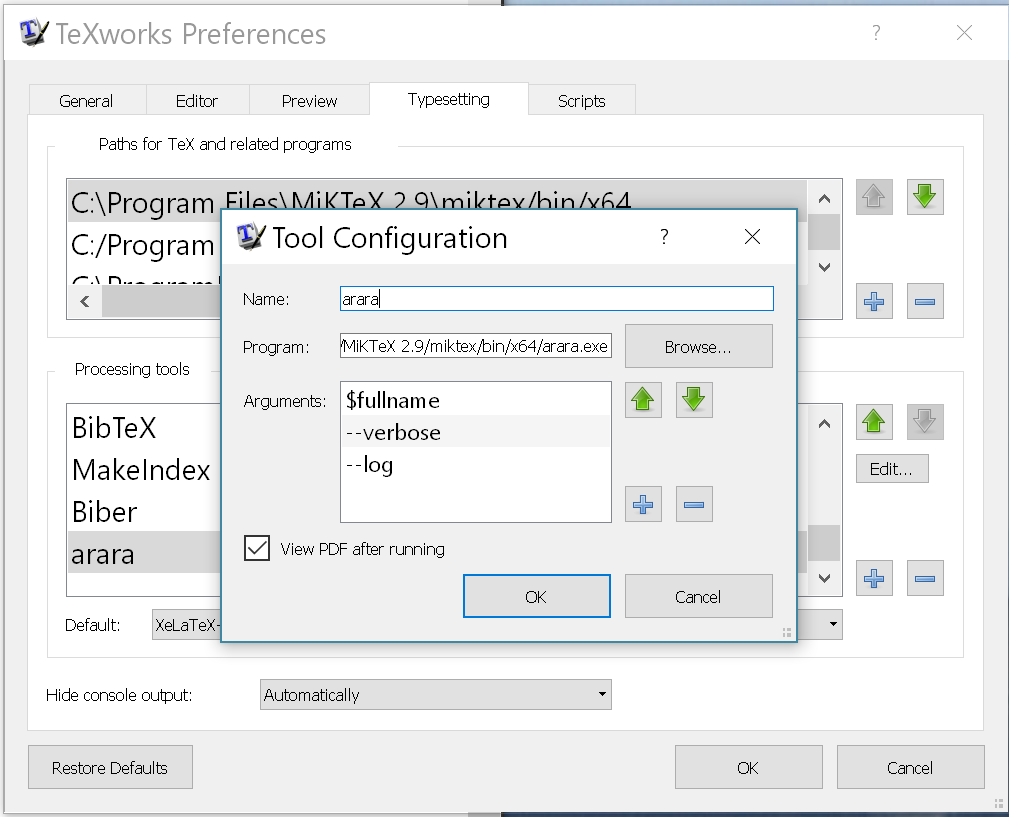
\includegraphics[scale=0.5]{figs/arara.png}
\caption{Java \texttt{Number} classes.}
\label{fig:java-number-classes}
\end{figure}

Boxed vs primitive arithmetic benchmark; 
int vs long vs float vs double vs Integer \ldots vs BigDecimal.


%-----------------------------------------------------------------
\setcounter{currentlevel}{\value{baseSectionLevel}-1}
\levelstay{Clojure}
\lstset{language=Clojure}

Clojure provides the primitive and boxed object numbers from Java,
except:
\begin{itemize}
  \item Full support for primitive type hints (eg for function arguments and
  return values) is only available for \lstinline|long| and \lstinline|double|.
  \item Idiomatic Clojure obscures whether primitive or boxed values will be
  used in any particular chunk of code (even more than recent versions  Java)
  Because of this, it is good practice to begin every namespace with
\begin{lstlisting}[
caption={[Boxed arithmetic warnings]}, label=unchecked-math,]  
(set! *unchecked-math* :warn-on-boxed)
\end{lstlisting}
which will generate compile-time warnings
\end{itemize}

Clojure adds rational numbers, which turn out to rarely be useful.\\
\lstinline|clojure.lang.Ratio| rational numbers
\lstinline|clojure.lang.BigInt|~\cite[p.~428]{Emerick2012ClojureProgramming}

